

One of the challenges in brain research is finding relationships between the physical structure of the brain and the way it functions. Structural information is gathered mainly through the use of imaging techniques as Magnetic Resonance Imaging (MRI), Computer Aided Tomography (CAT) or Positron Emission Tomography (PET). Other methods measure the electrical activity of the brain, as in Electro-Encephalography  (EEG) or Magneto-Encephalography (MEG). Transcranial Magnetic Stimulation (TMS) is a technique where cells are stimulated using a rapid changing magnetic field, which in turn generates an electrical field inside the neurons, the effects of this stimulation are afterwards measured elsewhere. 

Traditionally research is done by formulating hypotheses and designing experiments to test such hypotheses. Next, recruiting subjects, performing the experiment on each of them and gathering data. Finally this data would be analyzes using statistical methods which provide evidence in favor or against the hypothesis. This methodology imposes limitations on how data is used. Usually data is only used once, which is a shame because gathering this data is expensive in time, effort and resources. 

In the past years there has been a shift towards gathering data in a more open fashion, and several public databases have appeared. There has been several improvements in the way data is collected, stored and shared, both at the technical level and at the policies level. Even inside small research groups, it has become usual to keep looking at the data after traditional hypothesis testing is complete. 

All of this is leading to a change in the way research is done. This is a shift from hypothesis driven research into data driven research. This also creates an increased need for exploratory analysis methods, where the ecosystem is dominated by methods created for confirmatory analysis. In this context new challenges appear. It is now necessary to manage, analyze and visualize data where the number of subjects is increased by orders of magnitude, as well as the measures available for each one. In this scenario it is hard to guarantee homogeneity on the data belonging to each subject. In several cases there are measures available for each subject at several points in time. 

The work-flow in this kind of analysis differs significantly from the traditional one. It requires iterating trough the data several times, looking at it from different points of view, searching for relevant subjects and measures, gathering details from individuals and performing group analyzes involving several measures. 

Similar scenarios have appeared in other domains, as in economy, terrorism prevention and business intelligence. The challenge is always extracting meaningful information from large and heterogeneous data-sets. Approximations to the problem often involve statistics, machine learning and databases together with efficient and intuitive interfaces and data visualizations. Visual Analytics has emerged as a discipline which attempts to integrate all of these areas with the objective of making an optimal use of the available data. Visual Analytics recognizes the human analyst as the most important element in the task, and focuses on letting the analyst work with freedom and efficiency and focused as much as possible on the data instead of the tools.

In this thesis visual analytics techniques are applied to the particular case of cohort studies in brain data. A model which abstracts and formalizes the elements of this task is proposed. This model can be adapted and applied to other domain where cohort-like data is found. The model is materialized in a software environment called BRAVIZ. This software was successfully used in a large brain study performed by the Kangaroo Foundation. The results are very encouraging and show that the proposed tools really helped the experts feel like they really owned their data and could move trough it freely and explore it as they liked. This created a pleasant experience where information, questions and hypotheses could be gathered from the data.


\section{Visual Analytics}

%Que es

Visual analytics is a discipline which "combines automated analysis techniques with interactive
visualizations for an effective understanding, reasoning and decision making on the basis of very
large and complex datasets" \autocite{cook_illuminating_2005}. It is based on the premise that computers and
human beings have different sets of skills which should complement each other. Modern
computing systems are able to store and operate on very large amounts of data.
Specifically data-mining, clustering, machine learning and complex statistical methods can be
applied to Terabytes of data using high performance computers or clusters. These
algorithms, however, are limited in that they lack the theoretical framework, context and critical
thinking abilities necessary to make sense of data, specially when searching for the unknown. 
On the other hand, domain experts have a very rich theoretical
background, expertise and intuition which allow them to grasp the meaning of data and to
make better decisions about the direction that the analysis should move to. 

In Visual Analytics an environment where humans and machines can work
together and communicate fluidly is proposed, such that the specific abilities of both are used
efficiently. Fluid communication is achieved through rich interactive
visualizations and friendly user interfaces.
The human visual system has a large capacity to process information when it is
represented in the appropriate way \autocite{ware_information_2004}. Data visualization has been studied
exhaustively in the last years and many efficient ways to represent large multidimensional
datasets have been designed \autocite{heer_tour_2010}. As
pointed by Ware: "`The best visualizations are not static images to be printed in books, but fluid,
dynamic artifacts that respond to the need for different views or for more detailed
information"' \autocite{ware_information_2004}, interactivity is a fundamental component of these systems. 
However,  these interactions should be
as simple and intuitive as possible, in order to allow the analysts to focus their attention on the
data itself \autocite{spence_information_2007} rather than on details of the tools. 

In a visual analytics system automatic data processing algorithms are combined with interactive data visualizations
inside a loop \autocite{keim_mastering_2010}. The goal of the loop is to extract knowledge from data. Yet again, this process
is much more efficient when automatic tools are combined with visualizations and therefore allowing the intervention of the
human expert at early stages. 

The benefits of visual analytics are more evident when dealing with large and complex datasets. In this case it is also important
to have an efficient data storage infrastructure which can drive all the interactive process. 

From all of the above it can be seen that visual analytics
has to be supported on several areas of knowledge, such as data mining, data management, perception and cognition, human-computer interaction and scientific and information visualization \autocite{keim_visual_2008}. Elements from all these areas have to be integrated smoothly in order to achieve the goal of keeping the analyst focused on the data. In many cases this means managing in the background details that are not relevant for the task at hand. The analyst is always the main character in visual analytics, and all the other components should serve him, and be adapted to its needs. Therefore studying the user, its way of working, and the particular analysis tasks is a requirement to design this kinds of systems. 
%Ejemplos


These concepts can be applied in several domain as law enforcement, business intelligence, city planning, network analysis and bio-informatics\footnote{Tarea: Buscar referencias}. In fact the framework can be applied everywhere there is a need to extract meaning from data, specially where data is large, heterogeneus, noisy, incomplete or unstructured. However because it is centered on the domain, and particular analysis needs, there can't be a single system that works on every domain. Actually the biggest contribution of visual analytics is recognizing the analyst as the most important element, and putting all these disciplines at his service in order to help him solve his analysis tasks. The analysts is always the one in control and the one who knows what is important and what isn't. The fact that the system should adapt to the system, and not the other way around \autocite{norman_design_2002} absolutely holds. 

\section{User Centered Design}

Creating systems that truly meet users' needs requires taking the user into account from the start. This may sound obvious, but is not. There are several examples of systems that are outstanding from a technical level but fail to be useful\autocite{norman_design_2002}. User centered design\autocite{baxter_understanding_2005}, proposes a methodology to efficiently consider the user as part of the design process. 

The principles of user-centered design are \autocite{baxter_understanding_2005}:

\begin{itemize}
	\item An Early Focus on Users and Tasks
	\item Empirical Measurement of Product Usage
	\item Iterative Design
\end{itemize}


Several techniques have been developed to address the first point. The point is to extract information about user needs, analysis tasks and use cases. This sounds simple but it is actually very complex to grasp the reality. The instruments available for this task include survey, interviews, focus groups and field studies. For more information about these methods refer to \autocite{baxter_understanding_2005} or \autocite{hartson_ux_2012}.

During the interaction with users several aspects must be taken into account. 
Some people argue that users don't really know what they want. There is some truth in this, because often users can't directly point you to what they want or need. They get so used to going through loops in their daily work, that they start to think of it as a natural step in the process. In order to go through this it is very important to pay attention and to ask questions. It is necessary to observe them working, the actual observed behavior is different to how it is narrated. During field visits pay attention to the surroundings, the environment also has a lot to say about how people work. If possible try to collect artifacts: pictures, paper forms, or screen-shots.

Pay special attention to hesitation, problems or barriers. For example in one of the labs we visited the researcher was showing us how to analyze some TMS data. One of the steps involving moving the file to the desktop. When asked about why, he told us that the next program would not work otherwise. This was natural for him, but it shouldn't be like that. This is an unnecessary steps that has a negative impact on productivity. Notice that users are human, and therefore they are unlikely to accept ignorance or problems. Special attention is required to detect this issues.

It is very important to avoid placing the designer ideas into the domain expert's mind. Questions must always be asked in an open form. For example instead of saying "`So what you are trying to do is .....?"', say "`Please elaborate on what you are doing"'. Users should not design, but they can give suggestions. Avoid asking directly "`What do you want?"' or "`What do you need?"', instead focus on collecting how the work is done now. During the first stages, limit to listen, observe and ask for details. Ideally the users should tell you stories about current and past work, specially the tricky cases. 

\smallskip

The second point focuses on evaluating usability of the product.  Early evaluations should involve real users and real applications to the best extent possible in order to detect problems and opportunities. These evaluations should be performed with potential users. They should look at the prototypes thoroughly and test which features are useful and which ones not so much. Evaluation processes are best if they can be done in a realistic scenario, using example data and tasks similar to the ones done on a day to day basis by the experts. If possible, quantitative and qualitative data should be collected. There is a high risk of involuntarily biasing the evaluation process, so measures must be taken to make it as honest and transparent as possible. 

For this task several techniques are also available, including: controlled experiments, think-aloud, survey, and Multidimensional In-depth Long Term Case studies \autocite{shneiderman_strategies_2006}.

\smallskip

The whole process is composed of several analysis, design and evaluation cycles as shown in figure \ref{intro_spiral}. The first cycles should be fast and produce low fidelity prototypes. While the later iterations are expected to last longer and produce high fidelity prototypes and even fully functional beta versions. 

\begin{figure}
\centering
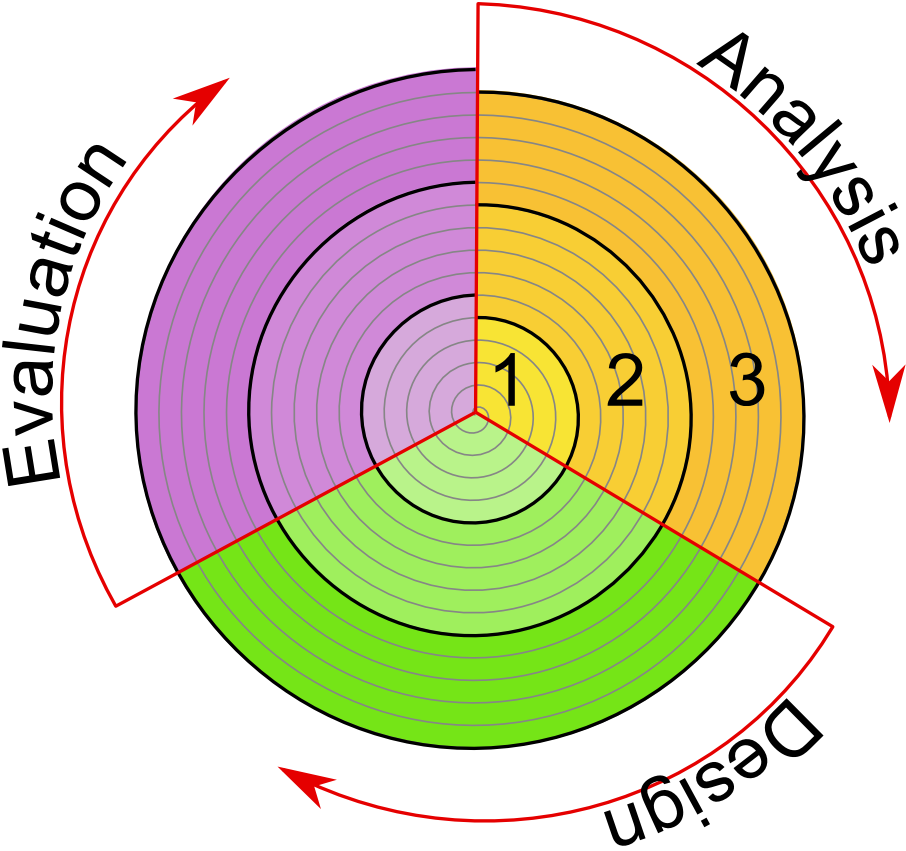
\includegraphics[scale=1]{espiral2.png} 
\caption{ \label{intro_spiral} The user centered design process}
\end{figure}

During the analysis phase, all the information gathered from the subjects should be sorted and analyzed. Patterns and common needs should be made evident, and design decisions should be made based on these observations. It is crucial that the proposed solution respects current standards and that it plays nice with current tools. They should also implement the language used by final users instead of the technical terms used inside.  Proposals should be materialized in prototypes which will be the prime matter for the evaluation phases. In these users get involved again in order to assess if the design is on the right track and making the necessary adjustments. During this process additional questions or use cases may emerge. Possible the need for additional information from users will appear. All of these information will be the input for the next iteration.

%Respect standards
%Play nice with current tools
%Language of the users
%Cite UX-book
%Be a listener
%Users hide ignorance, thy try to appear smart

\section{Exploratory and Confirmatory Analysis}

The usual way of doing science is derived from the scientific method. It consists of raising hypotheses, designing experiments that will provide evidence on the hypotheses, performing such experiments and collecting the data, and finally analyzing the data using statistical techniques. When done right and rigorously this method can help us increase our understanding of the world. However there are also some problems in it. First, hypotheses should be raised based on observation and previous knowledge, and this itself is not a trivial task. Data in this method is collected exclusively with the goal of testing a given hypotheses, and most of the time the data is archived after this is accomplished. Traditionally the statistical methods used were based on null hypothesis testing. This methods by themselves have also caused several problems like publication bias \autocite{ioannidis_why_2005}, and the dangers of using p-values without completely understanding them \autocite{halsey_fickle_2015}, \autocite{nuzzo_scientific_2014}, \autocite{woolston_psychology_2015}. Notice that the problem is not limited to the classical p-values from statistical inference \autocite{gelman_so-called_2011}, the problem raises from wanting to find a single number that represents the whole research, reality is seldom that simple.    

This doesn't mean that confirmatory research is not useful, in fact it is necessary, but it has to be done right. Some of the issues can be solved by avoiding p-values or similar statistics and by taking in reproducible research practices. This means, publishing the totality of the data and computer scripts used in the analysis in such a way that third parties can verify and play with the results. 

The issue of discovering hypotheses can be addressed by exploratory or data-driven research. It is well known that today the amount of data collected is enormous. Fortunately, plenty of this data is public. If open research practices catch up, the amount of available interesting data-sets will magnify. All of this data provides a mine where hypotheses can be found and preliminary tests can be done before compromising on the rigor of confirmatory analysis. 

The human genome project\footnote{missing citation} is a good example of how open data can benefit science overall. A important part of this project was creating a public database of genetic data, where all authors who wanted to publish were required to send their sequences. This created a repository that could be searched and analyzed by anyone, resulting in the discovery of new interesting patterns and hypotheses.

In economics it is usual to see research (for example \autocite{levitt_freakonomics_2006}) based entirely on public data, like results from census or social networks data. In fact most of the world governments are creating open data policies, that make important amounts of data available for anyone to explore.

In brain research several projects are collecting large data-sets and making them available for the public to explore, such as the human connectome project\autocite{rosen_human_2010} and ADNI\autocite{jack_alzheimers_2008}. There are also a vast amount of open source tools and frameworks that can make reproducible research a reality. These will be covered in detail on chapter \ref{chap_state_of_the_art}. Private data-sets collected inside an organization can also be used as the input for exploratory research, as will be seen in chapter \ref{chap_kmc400}.

Even though large amounts of data is becoming available, the methods and tools necessary for efficiently exploring it are just starting to appear. This thesis proposes a model and tool for exploring large data-sets in brain research. It is based on the visual analytics principles, and followed a user-centered design methodology.

%Confirmatory analysis

%Exploratory analysis

%Economia, como freakanomics, datos de censos, datos publicos.

%Human Genome

%Data Driven Research

%Reproducible research

%Open Data

%Critiques to P-Values

%Publication Bias


\section{Objectives}

This thesis will address the challenge of designing tools for supporting exploratory analyzes with cohort data, applying the principles of visual analytics and human centered design. A model of how data and analysis tasks interacts in this scenario is the center piece. From it, it is possible reason about the problem and design better solutions. BRAVIZ is a prototype based on this model and on our work with end users. This prototype was used in a large study, and it had a significant impact of how researchers use their data. The punctual objectives of the thesis are

%Objectives
\begin{itemize}
\item Create a model of cohort data and visual analysis tasks that can be used to think about the exploratory analysis problem in cohort data.

\item Implement a prototype based on the model to validate it in the brain studies case.

\item Evaluate the prototype with a real brain study, real users and real tasks.

\end{itemize}

The project is further concentrated on multi-disciplinar teams as users. These teams should contain people with expertise on image data, and there should be an interest to look at the subjects as a whole instead of at different dimensions independently. These interactions withing the different specialists are considered inside the model. 

%Hypotheses
The working hypothesis is that  current tools are not ideal for exploratory analysis in cohort brain data. Exploratory analysis is more efficient when only specific functionality is exposed to the user and the rest is handled underneath. In particular repetitive tasks and complexities in data access are barriers. 

In order to assess this it is required to find out several aspects of the neuroscience research community. How often is exploratory analysis done? If not often, then why? How can it be made more efficient? How can it involve more people? What are the main bottlenecks that limit exploratory analysis? We will only address technological bottlenecks, but certainly other types exist, for example cultural or political. With these work we hope to make exploratory analysis more viable, which in turn means making better use of the data and hopefully encourage more researchers to adopt reproducible research, open data, open source and in general, a more collaborative model for science.

%Research questions


%What are the requirements for visual exploration in cohorts?
%What are the most important tasks?
%What is the appropriate level of detail?
%How can multiple points of view be supported?






